\documentclass[letterpaper, 12pt]{article}

\usepackage{hyperref}
\usepackage{pgfplots}
\usepgfplotslibrary{fillbetween}

\title{Basics of Economics}
\author{Alvin Lin}
\date{Principles of Microeconomics: August 2016 - December 2016}

\begin{document}

\maketitle

\section{Elasticity}
When supply decreases, the equilibrium price rises and the equilibrium
quantity decreases. The amount that the price and quantity increase and
decrease depends on the \textbf{responsiveness} of the quantity demanded of
a good to a change in its price.

\subsection{Price Elasticity of Demand}
One candidate for a measure of the responsiveness is the slope of the demand
curve. If the demand curve is flat, then the quantity decreases by a lot in
response to a relatively small increase in the price. If the demand curve is
steep, then the quantity decreases by a relatively small amount in response to
a relatively large increase in the price. Since the responsiveness depends on
the slope, we want a units free measurement when comparing it.
\[ E_{P} = \frac{\%\Delta Q}{\%\Delta P} \]
The elasticity in demand is equal to the percentage change in quantity demanded
over the percentage change in price.
\[ \%\Delta Q = \frac{Q_{new}-Q_{old}}{Q_{average}}\times 100 \]
\[ Q_{average} = \frac{Q_{new}+Q_{old}}{2} \]
\[ \%\Delta P = \frac{P_{new}-P_{old}}{P_{average}}\times 100 \]
\[ P_{average} = \frac{P_{new}+P_{old}}{2} \]
\[ E_{P} = \frac{\frac{Q_{new}-Q_{old}}{Q_{average}}\times 100}
            {\frac{P_{new}-P_{old}}{P_{average}}\times 100} = \]
\[ \frac{Q_{new}-Q_{old}}{P_{new}-P_{old}}\times
   \frac{P_{average}}{Q_{average}} \]
\[ \frac{Q_{new}-Q_{old}}{P_{new}-P_{old}}\times
   \frac{\frac{P_{new}+P_{old}}{2}}{\frac{Q_{new}+Q_{old}}{2}} \]
\[ \frac{Q_{new}-Q_{old}}{P_{new}-P_{old}}\times
   \frac{P_{new}+P_{old}}{Q_{new}+Q_{old}} \]

\subsubsection{Practice Problem}
Suppose you have been hired by the government to figure out a tax that will
reduce cigarette smoking by \( 25\% \). After a careful study, you decide
that the price elasticity of demand for cigarettes is \( E = -0.5 \). What
tax do you recommend to the government?
\[ E_{P} = -0.5 = \frac{\%\Delta Q}{\%\Delta P} = \frac{-25}{\%\Delta P} \]
\[ \%\Delta P = \frac{-25}{-0.5} = 50 \]
\begin{center}
  50\% tax on cigarettes.
\end{center}

\subsubsection{Ranges of Price Elasticity}
\begin{itemize}
  \item Elasticity can range from \( 0 \) to \( \infty \).
  \item Demand can be elastic (very responsive). \( |E_{P}| > 1 \)
  \item Demand can be inelastic (not very reponsive). \( |E_{P}| < 1 \)
  \item Demand can be unit elastic. \( |E_{P}| = 1 \)
\end{itemize}
\[ E_{P} \in \bigg(-\infty, -1\bigg): Elastic \]
\[ E_{P} \in \bigg(-1, 0\bigg]: Inelastic \]

\subsubsection{Practice Problem: \(|E| > 1 \)}
The percentage change in Q is greater than the percentage change in P.
For example, if the prices of movies increase from \$20 to \$30, and the demand
decreases from 1000 to 500.
\[ E_{P} = \frac{Q_{new}-Q_{old}}{P_{new}-P_{old}}\times
       \frac{P_{new}+P_{old}}{Q_{new}+Q_{old}} \]
\[ E_{P} = \frac{500-1000}{30-20}\times\frac{30+20}{500+1000} \]
\[ = \frac{-500}{10}\times\frac{50}{1500} = -\frac{5}{3} \]
\[ |E_{P}| = \frac{5}{3} \]

\subsubsection{Factors that Influence the Elasticity of Demand}
The elasticity of demand can change depending on different factors.

\paragraph{Closeness of Substitutes:} The demand for a good is elastic if a
substitute for it is easy to find. The demand for a good is inelastic if
substitutes are hard to find. \textbf{Necessitites}, such as food or housing,
generally have inelastic demand while \textbf{luxuries} generally have elastic
demand. The availability of substitutes depends on type of good and how
broadly or narrowly the good is defined.

\paragraph{The Proportion of Income Spent on the Good:}
The greater the proportion of income spent on the good, the greater the impact
of a price increase on the amount that people can afford. A higher proportion
spent on the good implies a more elastic demand.

\paragraph{Time Elapsed Since Price Change:}
More time elapsed implies more elastic demand.

\subsubsection{Price Elasticity Along a Linear Demand Curve}
\begin{center}
  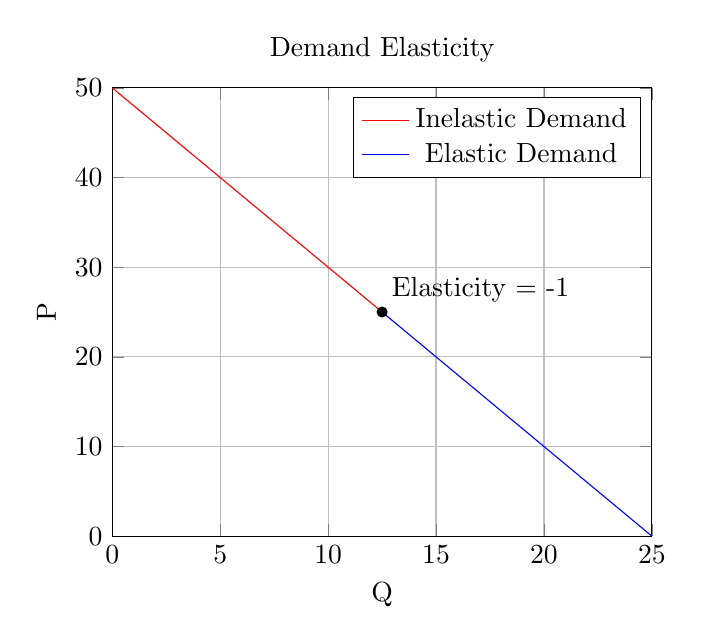
\begin{tikzpicture}
    \begin{axis} [
      title={Demand Elasticity},
      xlabel={Q},
      ylabel={P},
      xmin=0, xmax=25,
      ymin=0, ymax=50,
      grid=both
    ]
      \addplot[color=red] coordinates { (0,50)(12.5,25) };
      \addlegendentry{Inelastic Demand}
      \addplot[color=blue] coordinates { (12.5,25)(25,0) };
      \addlegendentry{Elastic Demand}
      \fill (12.5,25) circle[radius=2pt];
      \draw (12.5,25) node[anchor=south west] {Elasticity\ =\ -1};
    \end{axis}
  \end{tikzpicture}
\end{center}

\subsubsection{Total Revenue and Elasticity}
A firm that sells a product obtains revenue from the sales. The total revenue
is the price of a good times the quantity sold.
\[ TR = P \times Q \]
If Starbucks sells a million lattes at \$4.00 each, then they make \$40,000,000
in total revenue. If they increase the price of lattes, then the quantity
demanded will go down.

\subsection{Income Elasticity of Demand}
Income elasticity is a measure of the responsiveness of the demand for a good to a change in income, ceteris paribus.
\[ E_{m} = \frac{\%\Delta Q}{\%\Delta M} \]
Like price elasticity of demand, this formula can be simplified to:
\[ E_{m} = \frac{Q_{new}-Q_{old}}{M_{new}-M_{old}}\times
           \frac{M_{new}+M_{old}}{Q_{new}+Q_{old}} \]

\subsubsection{Practice Problem 1}
Income rises from \$750 a week to \$1250 a week, while the quantity demanded
of Kraft Dinner decreases from 7 boxes a week to 3 boxes a week. What is the
elasticity?
\[ E_{m} = \frac{Q_{new}-Q_{old}}{M_{new}-M_{old}}\times
           \frac{M_{new}+M_{old}}{Q_{new}+Q_{old}} \]
\[ \frac{3-7}{1250-750}\times\frac{1250+750}{3+7} \]
\[ \frac{-4}{750}\times{2000}{10} \]
\[ = -\frac{8}{5} \]

\subsubsection{Practice Problem 2}
Income rises from \$750 a week to \$1250 a week, while the quantity demanded of
salmon fillet rises from 1 pound a week to 2 pounds a week. What is the
elasticity?
\[ E_{m} = \frac{Q_{new}-Q_{old}}{M_{new}-M_{old}}\times
           \frac{M_{new}+M_{old}}{Q_{new}+Q_{old}} \]
\[ \frac{2-1}{1250-750}\times\frac{1250+750}{2+1} \]
\[ \frac{1}{500}\times\frac{2000}{3} \]
\[ = \frac{4}{3} \]

\subsubsection{Ranges of Income Elasticity}
If income elasticity is position and greater than one, it is income elastic.
If income elasticity is negative and less than minus one, it is income elastic.
\textit{A one percent increase in income results in a greater than one percent
increase in quantity demanded}. \par
An income elasticity between -1 and 1 means the it is income inelastic.

\subsection{Cross Price Elasticity of Demand}
Cross elasticity is a measure of the responsiveness of the demand for a good
to changes in the price of a \textit{substitute} or \textit{complement},
ceteris paribus.
\[ E_{X,Y} = \frac{\%\Delta Q_{X}}{\%\Delta P_{Y}} \]
\[ E_{X,Y} = \frac{Q_{X}^{new}-Q_{x}^{old}}{P_{Y}^{new}-P_{Y}^{old}}\times
             \frac{P_{Y}^{new}+P_{Y}^{old}}{Q_{X}^{new}+Q_{x}^{old}} \]

\subsubsection{Practice Problem}
When the price of Adidas increases from \$100 to \$120, the quantity demanded
of Nikes increases from 1 million to 3 million per year.
\[ E_{X,Y} = \frac{3-1}{120-100}\times\frac{120+100}{3+1} \]
\[ \frac{2}{20}\times\frac{220}{4} \]
\[ = \frac{11}{2} \]

\subsubsection{Ranges of Cross Price Elasticity}
The magnitude of the elasticity indicates how closely related the goods are.
A large positive elasticity indicates the goods are closely related substitutes.
A small positive elasticity indicates they are substitutes but not closely
related. A small negative elasticity indicates they are complements but not
closely related and a large negative elasticity indicates they are close
complements.
\begin{center}
  \begin{tabular}{|c|c|c|}
    \hline
    Sign & Magnitude & \\ \hline
    -    & large     & close complements\\ \hline
    -    & small     & complements \\ \hline
    +    & large     & close substitutes \\ \hline
    +    & small     & substitutes \\ \hline
    0    & 0         & not related \\ \hline
  \end{tabular}
\end{center}

\subsection{Elasticity of Supply}
Elasticity of Supply is a measure of the responsiveness of the quantity supplied
of a good to changes in the price of the good, ceteris paribus. The formula
follows the same form, but \( Q \) is now a quantity of supply instead of a
quantity of demand.
\[ E_{S} = \frac{\%\Delta Q}{\%\Delta P} \]
\[ E_{S} = \frac{Q_{new}-Q_{old}}{P_{new}-P_{old}}\times
           \frac{P_{new}+P_{old}}{Q_{new}+Q_{old}} \]

\subsubsection{Ranges of Elasticity of Supply}
\begin{itemize}
  \item Supply is perfectly inelastic. \( E_{S} = 0 \)
  \item Supply is inelastic. \( E_{S} \in (1, 1) \)
  \item Supply is unit elastic. \( E_{S} = 1 \)
  \item Supply is elastic. \( E_{S} \in (1, \infty) \)
  \item Supply is perfectly elastic. \( E_{S} = \infty \)
\end{itemize}

\subsubsection{Factors that Influence the Elasticity of Supply}
The elasticity of supply can change depending on different factors.

\paragraph{Resource Substitution Possibility:}
Some goods can only be produced using rare resources. These have inelastic
supply curves. Other goods are produced using resources that can be used in
a wide variety of production tasks.

\paragraph{Time Frame for the Supply Decision:}
Short run supply determines the changes to supply that can occur when some of
the factors of production remain fixed. A firm can layoff or hire new workers
in the short run. But it may not be able to build a larger factory. Long run
supply determines the changes in supply that are possible when all factors are
variable.

\subsubsection{Elasticity Along a Linear Supply Curve}
\[ E_{S} = \frac{1}{slope}\times\frac{P_{average}}{Q_{average}} \]
\begin{center}
  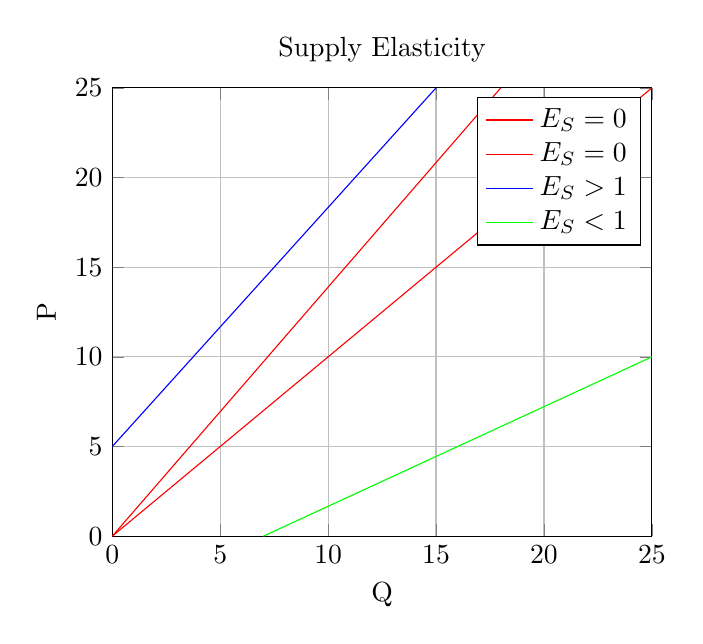
\begin{tikzpicture}
    \begin{axis} [
      title={Supply Elasticity},
      xlabel={Q},
      ylabel={P},
      xmin=0, xmax=25,
      ymin=0, ymax=25,
      grid=both
    ]
      \addplot[color=red] coordinates { (0,0)(25,25) };
      \addlegendentry{\( E_{S} = 0 \)}
      \addplot[color=red] coordinates { (0,0)(18,25) };
      \addlegendentry{\( E_{S} = 0 \)}
      \addplot[color=blue] coordinates { (0,5)(15,25) };
      \addlegendentry{\( E_{S} > 1 \)}
      \addplot[color=green] coordinates { (7,0)(25,10) };
      \addlegendentry{\( E_{S} < 1 \)}
    \end{axis}
  \end{tikzpicture}
\end{center}
Any supply curve that passes through the origin has an elasticity of 1.

\begin{center}
  You can find all my notes at \url{http://omgimanerd.tech/notes}. If you have
  any questions, comments, or concerns, please contact me at
  alvin@omgimanerd.tech
\end{center}

\end{document}
